\chapter{需求分析与概要设计}

\section{需求分析}
\label{sec:requirements-analysis}

本视频编辑系统的需求分析基于技术可行性研究,主要涵盖目标用户分析、功能性需求分析与非功能性需求分析。

\subsection{用户分析}

本系统的目标用户分析如表~\ref{tab:system-users}所示。一方面该系统面向对最新人工智能技术感兴趣的研究者及普通用户,
需要提供简洁易用的界面和友好的交互体验;另一方面该系统面向实验室研究者,为他们提供了解用户真实需求的渠道,
包括相关的数据统计和分析功能。


\begin{table}
    \centering
    \bicaption{目标用户分析}{System Users Analysis}
    \label{tab:system-users}
    \resizebox{\linewidth}{!}{
    \begin{tabular}{cl}
        \toprule
        目标用户   &  用户特征与期望       \\
        \midrule
        专业人工智能研究人员 & 对算法研究较深,希望方便地得到已有工作成果的编辑结果用于对比或研究\\
        对算法感兴趣的非从业者 & 缺乏项目部署的理论基础,但又期望了解到最新研究成果,尝试最新算法的效果 \\
        本实验室的研究人员 & 期望将实验室算法部署到实际应用中,方便实验室成员获取用户反馈与需求 \\
        \bottomrule
    \end{tabular}
    }
\end{table}

\subsection{功能性需求分析}

在功能性需求方面,首先,多模态视频编辑功能应支持文本指令驱动、参考图像风格迁移、虚拟换装和光照调整等多种编辑方式,
允许用户自定义上传视频与编辑提示。其次,考虑到编辑过程需要预处理以及多轮训练,
系统无法实时的生成结果,因此需要在结果生成后通知用户并允许用户查看。最后,作为实验室算法的展示平台,系统需要
允许管理员用户导出统计信息以供研究使用。

\subsection{非功能性需求分析}

本系统的研发初衷是希望利用先进算法为用户提供方便快捷的编辑体验,同时作为实验室的展示平台与反馈信息来源,因此需要
在用户体验、数据安全、可维护性上满足用户需求。

\subsubsection{用户体验}

系统需要提供简洁易用的界面,包括友好的交互体验、合理的布局、外观的协调等,以方便用户快速上手。需要
避免过多的弹窗、信息等,以免干扰用户操作;同时,也需要在必要的时候提供提示与帮助信息,以帮助用户更好地使用系统。

\subsubsection{数据安全}

系统需要具备较高的安全性,应当采取的措施包括用户认证、数据库信息加密、前后端分离、
API接口鉴权等。另外由于系统部署在学校内网无法直接通过外网访问,需要网络地址转换(NAT)技术提供访问支持,
应当确保地址转换中网关能有效地阻止外部攻击。

\subsubsection{可维护性}
此外,系统应该具有较好的可维护性,包括代码规范、模块化设计、应用文档编写等,以方便后续的维护和升级。

\section{概要设计}

系统概要设计的主要任务是将一个复杂的系统按功能划分成模块,确定每个模块的功能及模块之间的调用关系;确定模块之间的
接口,即模块之间的数据传递方式。另外,根据系统涉及到的实体与实体间的关系,设计数据库的表结构。

\subsection{架构设计}

根据第一节所述的需求分析,我们采用分层微服务架构,结合事件驱动的设计模式,将系统划分为客户端层、服务层、数据层,如~\ref{fig:system_structure}所示。

客户端层通过组件管理、页面渲染提供响应式用户界面,并通过对服务层微服务的api调用处理用户交互事件;

服务层由Flask微服务集群组成,负责处理客户端请求,并与数据层通信进行数据存储和检索。服务层具体包括用户服务提供用户的注册、登录、找回密码等服务;
管理员服务提供数据统计与导出服务;编辑服务提供文件的上传、任务的上传与查询、任务的分发等服务。

数据层使用MySQL数据库存储用户信息、任务信息和编辑结果,使用Redis数据库存储任务队列和任务状态。

\begin{figure}[ht]
    \centering
    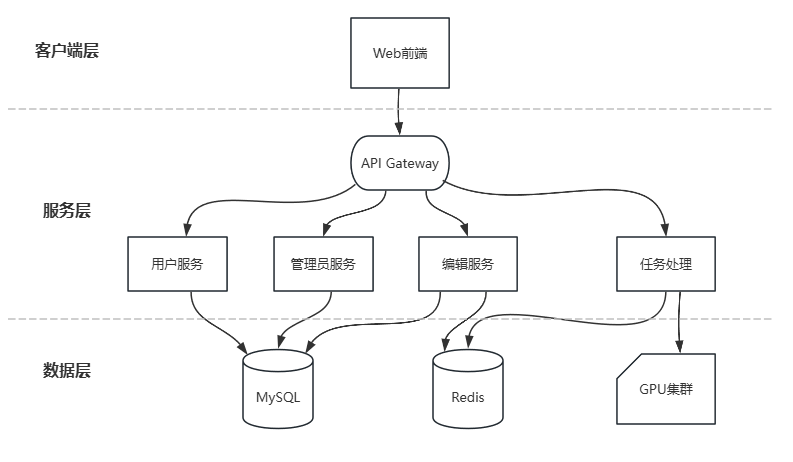
\includegraphics[width=0.6\textwidth]{source/img/system_structure.png}
    \bicaption{系统架构图}{System Architecture Diagram}
    \label{fig:system_structure}
\end{figure}

\subsection{4+1概要视图}

“4+1”视图是由Philippe Kruchten在1995年提出的一种软件架构描述方法。它将软件架构划分为四个视图,
包括逻辑视图、开发视图、物理视图和过程视图,以及一个场景视图。每个视图关注系统的不同方面,通过提供特定的抽象层次,
能够全面地描述系统的架构。场景视图关注系统的使用场景和用户需求,描述系统在特定场景下的行为和响应,我们已经在第一节
中详细地讨论过,下面我们着重通过其它四个视图来描述系统的架构设计。

\subsubsection{逻辑视图}

\subsubsection{开发视图}

\subsubsection{进程视图}

\subsubsection{物理视图}

\subsection{数据库设计}

根据需求分析,我们设计了用户表、任务表和编辑结果表,如~\ref{fig:database_design}所示。考虑到文件管理的需要,
我们在文件相关的表中添加了过期时间字段,以方便后续的文件清理工作。

\begin{figure}[ht]
    \centering
    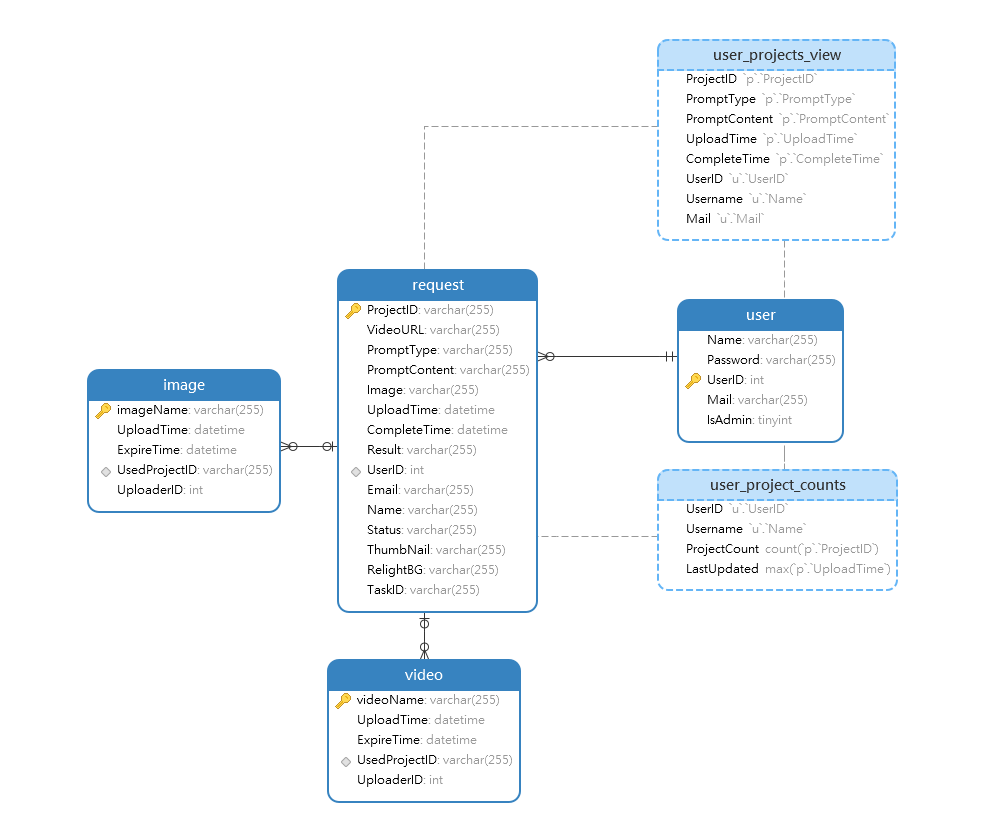
\includegraphics[width=0.6\textwidth]{source/img/database_design.png}
    \bicaption{数据库ER图}{Database ER Diagram}
    \label{fig:database_design}
\end{figure}
